\documentclass[../main.tex]{subfiles}

\begin{document}
\begin{problema}
	Un atleta está parado en la cima de una montaña cuya pendiente hace
	un ángulo \(\phi\) en la horizontal, como se muestra en la figura.
	¿A qué ángulo \(\theta\) debe lanzar una pelota de manera
	que el alcance sea máximo?

	\begin{figure}[htp]
		\centering
		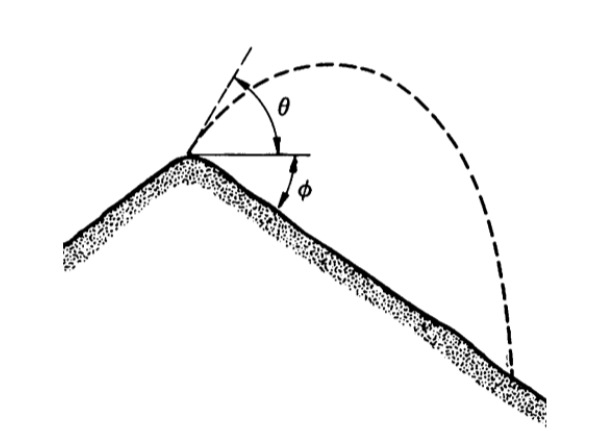
\includegraphics[scale=.4,trim={2cm 1cm 1.2cm 1.2cm}, clip]{../figs/problema_02.jpg}
	\end{figure}
\end{problema}
\end{document}
